%%%%%%%%%%%%%%%%%%%%%%%%%%%%%%%%%%%%%%%%%%%%%%%%%%%%%%%%%%%%%%%%%%%%%%%%%%%%%%%%
% Author : Jan Seibert, Tomas Polasek (template)
% Description : Seventh exercise in the Introduction to Game Development course.
%   It deals with the creation of a Game Design Document, presenting a short 
%   pitch for a potential game project.
%%%%%%%%%%%%%%%%%%%%%%%%%%%%%%%%%%%%%%%%%%%%%%%%%%%%%%%%%%%%%%%%%%%%%%%%%%%%%%%%

\documentclass[a4paper,10pt,english]{article}

\usepackage[left=2.50cm,right=2.50cm,top=1.50cm,bottom=2.50cm]{geometry}
\usepackage[utf8]{inputenc}

% Hyper-Text References
\usepackage{hyperref}
\hypersetup{colorlinks=true, urlcolor=blue}

% Drawing Images and Graphs
\usepackage{tikz}
\usepackage{pgfplots}

% Page Utilities
\usepackage{graphicx}

% Image Sub-Captions
\usepackage{subcaption}

\newcommand{\ph}[1]{\textit{[#1]}}

\title{%
Game Pitch Document%
}
\author{%
Jan Seibert (xseibe00)%
}
\date{18.12.2023}

\begin{document}

\maketitle
\thispagestyle{empty}

{%
\large

\begin{itemize}

\item[] \textbf{Title:} Otari

\item[] \textbf{Genre:} Battle Royale

\item[] \textbf{Style:} 3D, Simple Graphics, Performance aimed

\item[] \textbf{Platform:} PC

\item[] \textbf{Market:} People who enjoy survival games

\item[] \textbf{Elevator Pitch:} Every player spawns with game-item that represents player's life. When you lose it, the game is over for you. You can hide it inside your base that you can build.

\end{itemize}

}

\section*{\centering The Pitch}

\subsection*{Introduction}
The main thing that differs Otari from other battle royale games is the ability to strategize and plan your game style more. It's not only about Loot\&Kill. To win you also have to build your base, secure it, upgrade it and make sure that your heart does not get lost.

\subsection*{Background}
I personally enjoy battle royale games, the adrenaline rush during the match is huge compared to other game genres. Although after some time it really gets repetitive and the your game style usually has to be very quick. Meaning that you do not have a lot of time to think about your next step. That is where big inspiration from game Rust comes in. I would like to combine Rust game features with typical Last Man Standing games to achieve slower game style.
The feature to build your own base and raid other player's bases makes the games style much more slower, you 
What lead you to The Game's basic idea? What are the inspirations -- other games (even physical), sports, events, etc. Is it a continuation of some long-going traditional genre? Are you trying to bring back something that worked in the past?

\subsection*{Setting}
The story set in a sci-fi future. Doctors have come up with an invention that makes a person immortal, the planet is therefore becoming critically overpopulated and the government is doing so-called purges every month. 100 randomly chosen people are sent into the Arena and if a person wants to survive, he has to survive. If you happen to become the Champion of the Arena, you are guaranteed not to be selected for one year.

\subsection*{Features}
The selling points of my game are basically average of a typical survival game and a typical battle royale game.
\newpage

\begin{figure}[h]

\centering
    
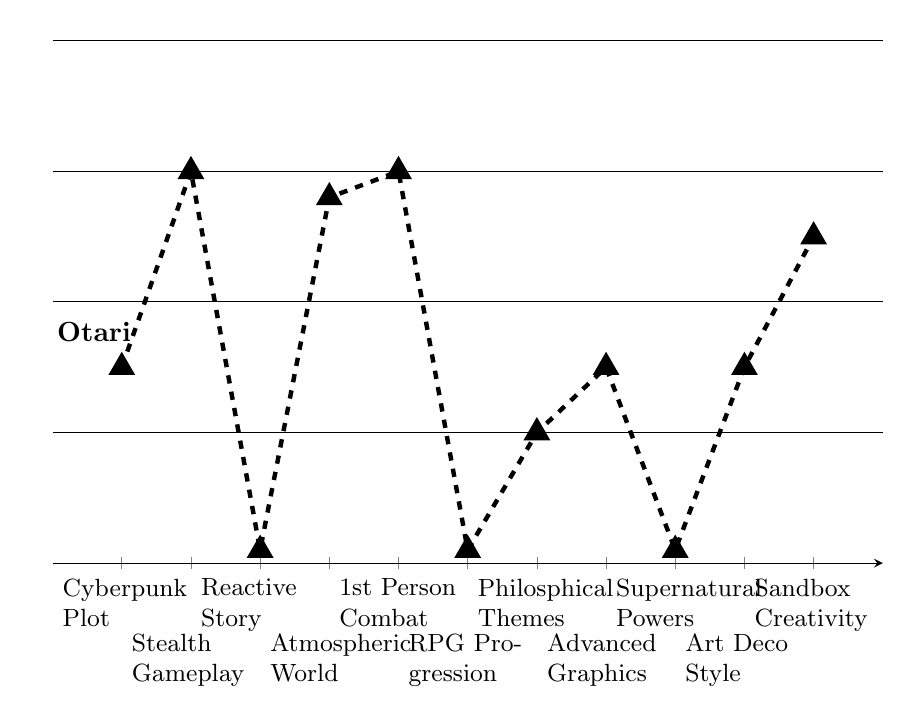
\begin{tikzpicture}[remember picture]%
\begin{axis}[
    domain=0:1, 
    clip=false, 
    ymin=0, xmin=0, ymax=4.1, xmax=12, 
    xtick={1,2,...,11}, 
    yticklabels={}, 
    xticklabels={Cyberpunk Plot, Stealth Gameplay, Reactive Story, Atmospheric World, 1st Person Combat, RPG Progression, Philosphical Themes, Advanced Graphics, Supernatural Powers, Art Deco Style, Sandbox Creativity}, 
    xticklabel style={yshift={-mod(\ticknum, 2) * 2em}, text width=1.5cm, font=\small}, 
    y tick style={draw=none}, 
    x axis line style={|-|}, 
    y axis line style={draw=none}, 
    axis lines=middle, 
    width=\linewidth, 
    height=0.3\paperheight
]

    \addplot [ultra thick, dashed, mark=triangle*, mark options={scale=2,solid}] coordinates {
        (1, 1.5)
        (2, 3.0)
        (3, 0.1)
        (4, 2.8)
        (5, 3.0)
        (6, 0.1)
        (7, 1.0)
        (8, 1.5)
        (9, 0.1)
        (10, 1.5)
        (11, 2.5)
    } node[above, yshift=5pt, xshift=-10pt, pos=0] {\textbf{Otari}};
    
	\draw [] (axis cs:{0,1}) -- (axis cs:{12,1});
	\draw [] (axis cs:{0,2}) -- (axis cs:{12,2});
	\draw [] (axis cs:{0,3}) -- (axis cs:{12,3});
	\draw [] (axis cs:{0,4}) -- (axis cs:{12,4});
\end{axis}
\end{tikzpicture}

\caption{Value graph for {Otari}}
\label{Fig:ValueGraph}
\end{figure}

\subsection*{Genre}
Battle Royale, Survival, First Person Shooter. Those are three main genres of this game, there are battle royale aspects - last man standing, one life. Survival aspects - base building, farming, looting, crafting.

\subsection*{Platform}
Otari is going to be released on PC mainly. But if the game will be be successful, there is a chace that it will be release on Playstation and Xbox as well.
Despite that, the PC release is going to be the most stable and the most updated and maintenanced release.
\newpage

\begin{figure}[h]
\subsection*{Style}
\centering

\begin{subfigure}{0.5\linewidth}
    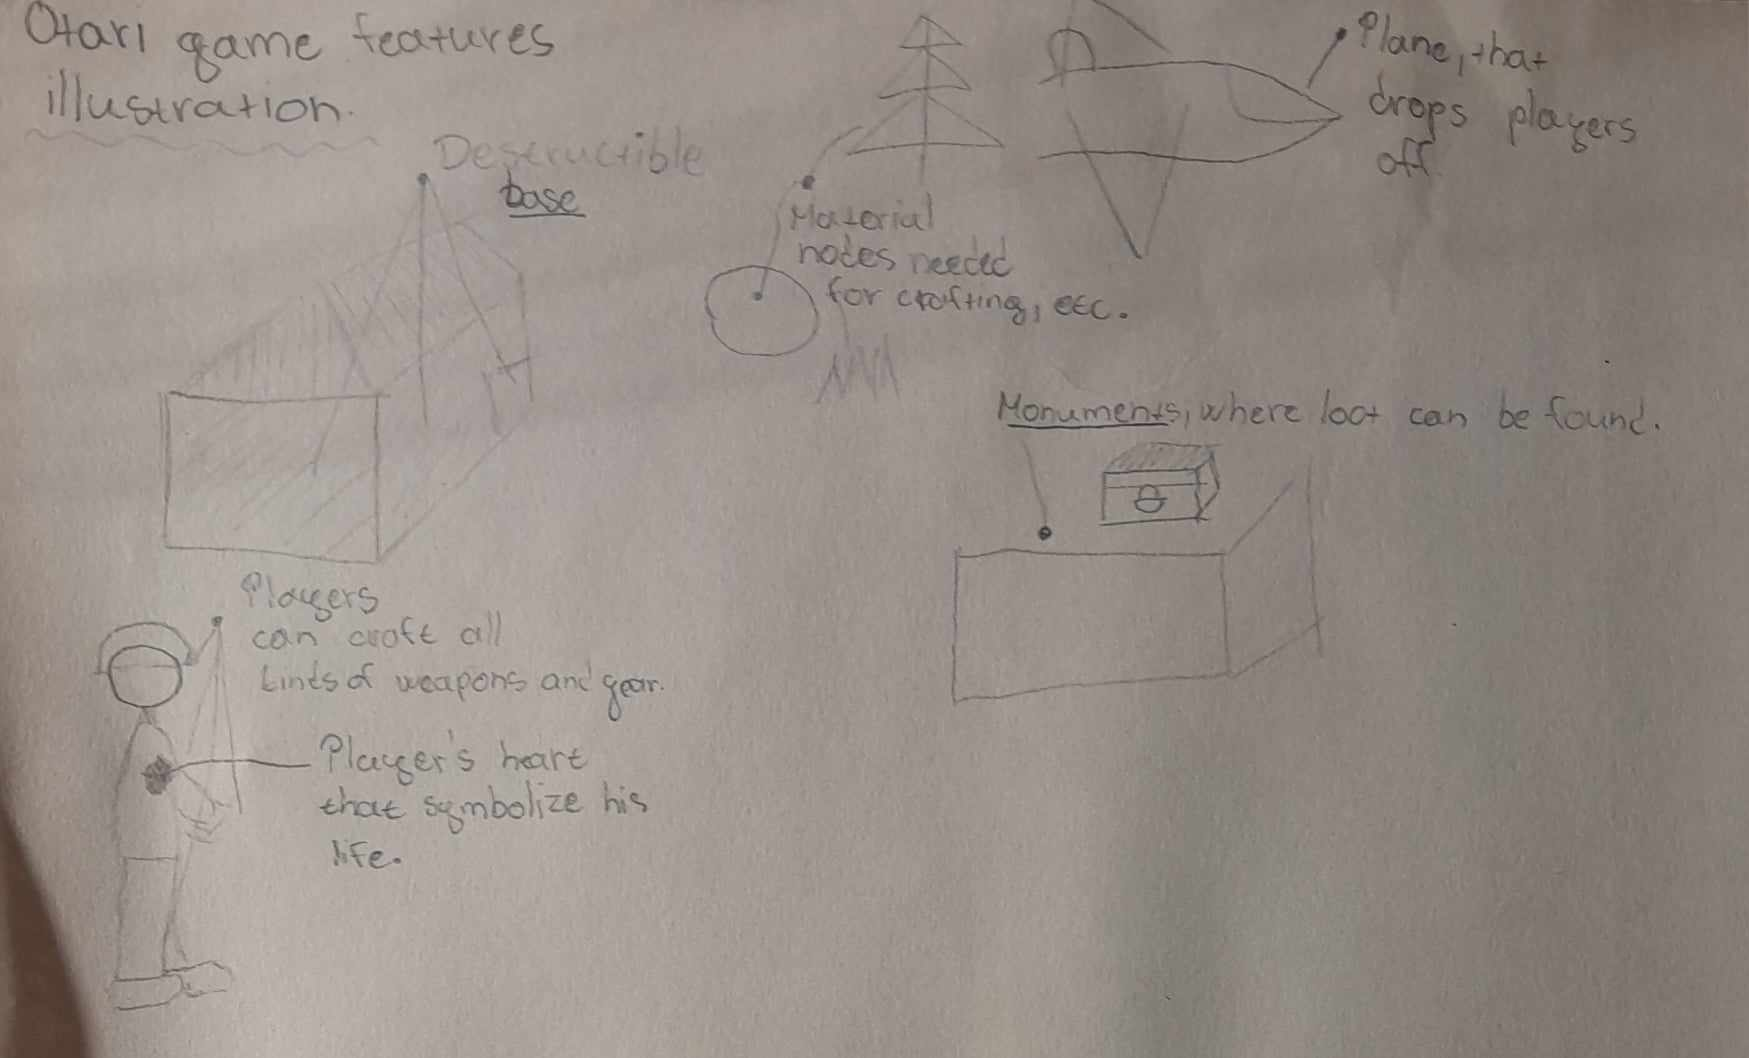
\includegraphics[width=\linewidth]{otari_sketch.jpg}
    \caption{Game features sketch 1a.}
    \label{Fig:Style1A}
\end{subfigure}
\par\bigskip
\begin{subfigure}{0.5\linewidth}
    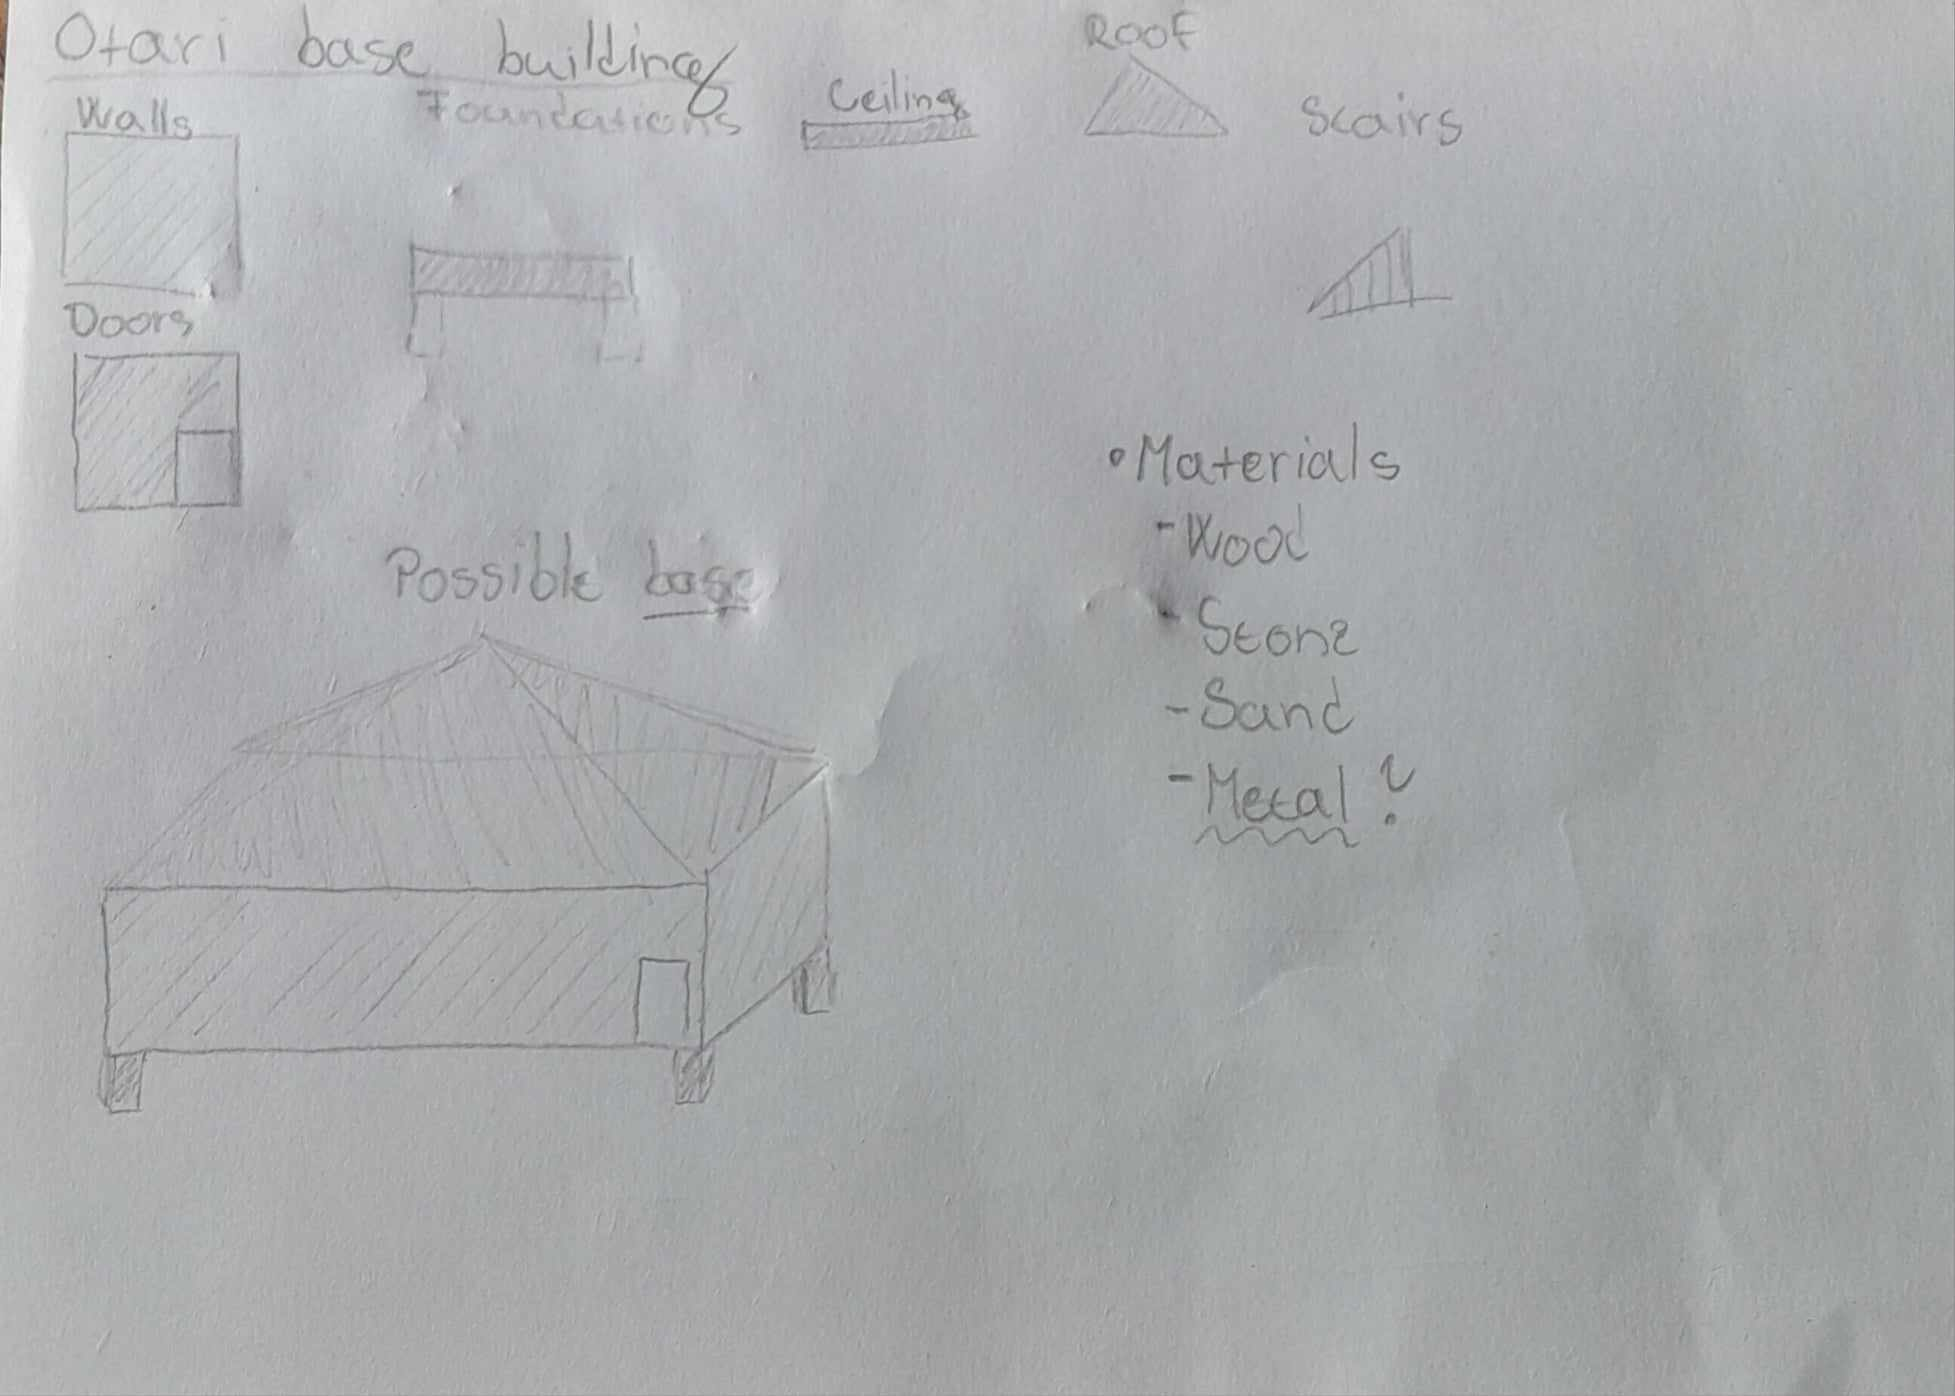
\includegraphics[width=\linewidth]{otari_base_sketch.jpg}
    \caption{Base building sketch 1b.}
    \label{Fig:Style1B}
\end{subfigure}
\par\bigskip
\begin{subfigure}{0.5\linewidth}
    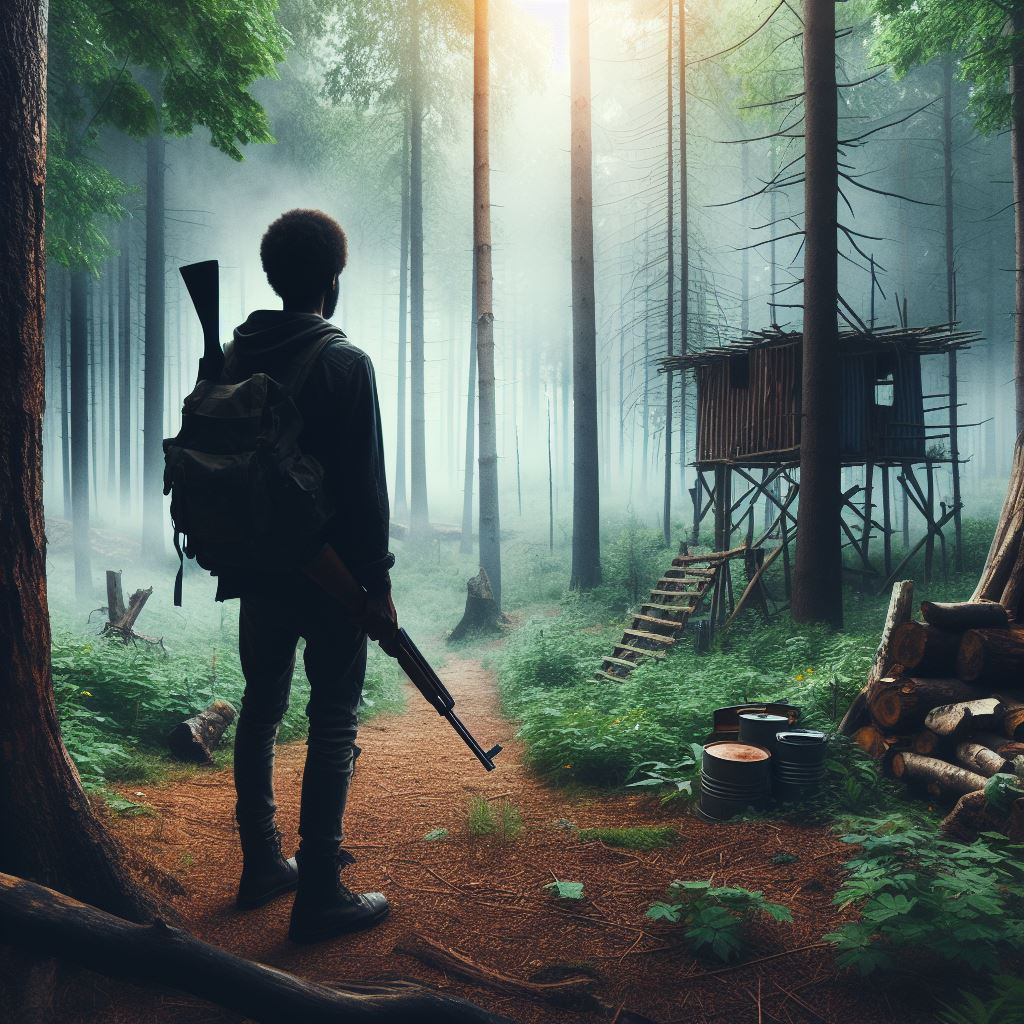
\includegraphics[width=\linewidth]{otari_ai.jpg}
    \caption{Possible look (AI GENERATED!) 1c.}
    \label{Fig:Style1C}
\end{subfigure}

\end{figure}

\end{document}
